\chapter{Deus et Eliseus Ascenderunt in Caelum}
\begin{center}
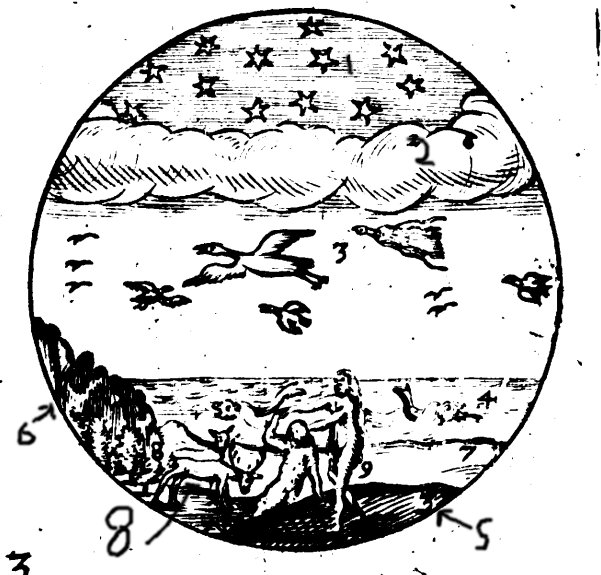
\includegraphics[scale=1.5]{World.png}
\end{center}

\section{Intended Audience}
This is intended for students who have completed Lectio 3 and 4 of Latin by the Natural Method and Chapter 4 of Lingua Latina Per Se Illustrata. There are 436 words in this chapter.

\section{Text}
Deus et Eliseus fīlius meus parvus ascendērunt in Caelum. Quōmodo Deus ascendit in caelum, sī sine corpore et sine locō est? Deus incarnātiōnem habet, quī ascendit in caelum et dēscendit ex caelō. Incarnātiō secundī hypostasis trīnitātis est Iēsus Chrīstus. Ergō, Deus (in incarnātiōne) et Eliseus fuērunt in nūbibus, quia ascendērunt in Caelō. Ēlīās etiam et Iēsus ascendērunt in caelum, sed Iēsus sōlus sedet ad manum dexteram Deī. 

In Caelō, Eliseus vīdit avēs, quae volāvērunt per nūbēs. Ubiubi Avis volāvit, movet āerem. Ubiubi Eliseus aspexit, Eliseus vīdit avēs et nūbēs. Quid nōn vīdit Eliseus? Angelōs nōn vīdit Eliseus. Cūr? Estne Angelī in Caelō cum Deō?  Angelī in caelō sunt. Caelum habet trēs significātiōnēs. Significātiō prīma est haec \: Ubi sunt nūbēs et avēs et sōl et lūna. Significātiō secunda \: Ubi sunt Angelī. Angelī nōn habent corpora nec locōs, sīcut Deus in essentiā, sed angelī in Caelō sunt. Tertia significātiō est ubi est Deus, in aeternō. Angelī nōn sunt in aeternō, sed in aevō. Angelī in aevō sunt quia creātiōnēs immortālēs sunt sed nōn ex aeternō. Ubiubi es, Omnēs Angelī illīc sunt. Ubiubi es, Deus tenet tē in ente et cum tē est. Utut fēcistī, Deus cum tē est. Utut es, Deus cum tē est, quia Deus dēdit ēns tibi. 

Dicāmus dē significātiōne prīmā. Caelum rotātur et ambit terram stantem in mediō. Quid est "ambit". Sīcut terra ambit sōlem, et nūbēs ambiunt terram. Iēsus fīlius Nun (Hic est Joshua anglice) ambit Jerichōnem septiēs. Quid est "rotātur"? Terra rotātur et ambit Sōlem. Sōl nōn rotātur, sed stat. Sōl, ubiubi est, fulget perpetuō in terrā. Sī nox in Eurōpā, diēs in Asiā. Nūbēs enim sunt in caelō, tamen sōl fulget, sed radiī nōn sunt in terrā. Radius est lūx quam mīsit Sōl in terrā. Eliseus nōn vīdit sōlem, sī in nūbibus dēnsīs est. Eliseus autem vīdit avēs, ergō nūbēs dēnsae nōn sunt, ergō Eliseus vīdit sōlem et radiōs eius. 

In nocte est Tenebrae. In nocte sunt Lūna et Stēllae. Stēllae micant in caelō et scintillant. Nōn lūna scintillat, quia nōn Stēlla est, sīcut carmen "Mīca, Micā Stēllam Parvam". Stēllae scintillant quia similis Scintillīs sunt. Scintilla est quae facit ignem, sīcut vir facit ignem cum scintillā. 

In māne, Sōl movet in Caelum. In vesperī, sōl movet ex caelō. In māne, vir labōrat cum aliīs hominibus. In māne, Stēllae nōn micant, nec Lūna splendet. In vesperī, Lūna splendet in Caelō, sed nōn stēllae. In vesperī, crepusculum est. In māne, nōn est crepusculum, sed aurōra et Dīlūculum. In vesperī, Discipulī Chrīstī ōrant Vesperās. In māne, ōrant Laudēs. Sōl fēcit lūcem, et ōrant Laudēs. Sōl fēcit tenebrās, et ōrant Vesperās. Deus amat Vesperās.
\footnote{\textbf{} = }